
\chapter{Finite Element Methods for the shallow water equations}
\label{eulerian_sw}


Due to the complexity of the geometry and the source terms is not possible to find an analytical solution for the SW equations, this explains the need to design strategies to find numerical solutions. In this chapter some numerical strategies with the FEM in an eulerian framework are explored.
The Eulerian frameworks are robust and very efficient for continuous problems. However, discontinuities and front tracking may require especial attention. Since in those physical phenomena flooding or moving shoreline may occur, the identification of the dry domain is a challenging problem for the Eulerian FEM.
Moreover, monotonic properties are especially interesting when partially wet domains are considered, since the water depth is a positive magnitude but, in general, numerical methods does not verify this property.

The SW equations have traditionally been modelled using finite volumes (FV) because of its advantages of stability and monotonicity. Given its geometric flexibility and its natural way to introduce high order schemes, the FEM has been applied too \cite{zien3,navon1979,navon1988}.
Halfway between FV and FEM, there is the discontinuous Galerkin (DG) technique \cite{ambati2007,khan2014,lee2019}. DG method has the advantages of the geometrical flexibility of the FEM and the stability of FV, but the introduction of high order DG schemes is not straightforward.
Since the FEM can exhibit spurious oscillations, different strategies such as stabilization, monotonic schemes or different order of polynomial interpolation can be explored \cite{hood1974,zien3,ortiz2012}.




%This research is focused in classical stabilized finite elements with an equal order interpolation for all the variables. We will explore the capabilities of the finite increment calculus (FIC) technique to develop stable formulations for the SW equations.

In this chapter, the general procedure for FEM is presented. Then, some stabilization techniques are explored: the FIC-based stabilization, the flux corrected technique and the gradient jump viscosity method. Finally, the stabilized formulation is applied to the Boussinesq modified equations. Several examples are provided to show the capabilities and limitations of each method.




\section{Galerkin weak formulation}


Given a residual


\section{Stabilized formulations for the shallow water equations}


Several families of stabilization methods can be found in the literature, usually applied to the convection-diffusion equations and the Navier-Stokes equations. The most relevant are SUPG \cite{brooks1982},
ASGS\cite{codina1998}, GLS \cite{hughes1989} and FIC\cite{onate1996,onate1998}.
Due to the hyperbolic character of the SW equations, a particular stabilization method for compressible flow or the Euler equations need to be developed.
The FIC approach is based on the incremental solution of a modified system of non-local governing equations accounting for higher order terms obtained by applying the balance laws in domains of finite size.
The FIC-based stabilization has been applied in conjunction with the FEM to convection-diffusion, incompressible flows, among other applications \cite{onate1998,onate2001}.
In those cases, where the convective term has an important role, a first order FIC term is enough to provide stability to the system.
However, the SW equations are governed by the convective term and the wave equation in a mixed formulation \cite{codina2008}. In consequence, the common derivation of the FIC-based stabilization is not enough to provide stability in all the range of applicability of the SW equations. 
A generalization of this method is proposed in order to provide a global stability for the SW equations.

Once global stability is achieved, local instabilities may appear near discontinuities, which are inherent to the supercritical flows.
A local shock capturing technique was initially proposed by Hughes \cite{hughes1986} and a review of shock capturing techniques can be found in Codina \cite{codina2011}.
Other possibilities of the FIC-based formulations are explored to provide a shock capturing stabilization \cite{cotela2016}.

Additionally, the dry domain requires an accurate modeling because the hyperbolic equations require positive water depth in all the domain.
Several authors have proposed different methods to solve the shallow water equations with moving shoreline. Leclerc et al. \cite{leclerc1990} proposed an Eulerian method. Later, Heniche et al. \cite{heniche2000} modified the method allowing the free surface to plunge under the topography.
Other authors developed a rough-porous layer \cite{candy2017,barros2011} or a modified depth integration \cite{defina2000}. These approaches introduce new physical parameters in the balance equations.
An Eulerian approach based on the work of \cite{leclerc1990} and \cite{heniche2000} is presented.






\subsection{Patch test}


Following Zienkiewicz \cite{zien1}, the patch test has been used as a first verification. The patch test is a basic verification which allows to verify the convergence. These tests have been developed imposing stationary solutions and obtaining the topography from the primary unknowns. The spatial domain $\Omega$ is a single element $e$.
Since the solution is stationary, the temporal domain is null and the test consist on the verification of zero accelerations.
Then, if the the solution belongs to the basis functions space, the test will pass analytically.
Otherwise, the test will pass asymptotically when the element is refined by subdivision of the domain ($h$-refinement). In that case, even if the element is not passing the test, the patch test is also useful since is checking the correctness of the implementation.

Several exact solutions have been applied to an element with size of $1m$. For the stabilized formulations a stabilization factor $\beta=0.01$ is used. The flux corrected solution depends directly on the stabilized formulation. If the solution belongs to the FE space, the obtained accelerations are less than $10^{-16}$, which is the round-off of machine precision.

\paragraph{Water at rest}
In this case, the free surface gradient and the velocity are zero. Some solutions can be built with that conditions, such as flat and non-flat topography, and bottom friction. In all the cases the accelerations are zero.

\paragraph{Slope in equilibrium}
This family of solutions verify constant water depth and constant velocity. The gravity terms (coming from the slope) are in equilibrium with the bottom friction terms. Several combinations are obtained with different directions of the slope and different Froude numbers, subcritical and supercritical.

\paragraph{Backwater analysis}
Finally, that family of analytical solutions, presents a constant flow rate where the gravity terms are in equilibrium with the bottom friction. But in that case, the primary unknowns do not belong to the FE space, since, either the velocity or the water depth are not linear. This test is passing asymptotically.


\subsection{Examples}


\section{The flux corrected transport for the shallow water equations}



\section{Quasi monotonicity preserving formulations}



\section{Stabilized formulation for the Boussinesq modified equations}




\subsection{Absorbing boundary conditions}

Es frecuente que que sea necesario acotar el dominio de estudio, imponiendo condiciones abiertas. Estas condiciones de contorno abiertas o radiantes han de permitir la salida de ondas, al mismo tiempo que garantizan la consistencia matemática del sistema de ecuaciones. Al mismo tiempo que la expresión matemática ha de garantizar la existencia de la solución, tambień ha de ser compatible con la disretización numérica empleada para el interior del dominio. Generalmente, se denomina condiciones de contorno radiantes a la formulación analítica y condiciones de contorno absorbentes al método numerico \cite{navon2004}.
Se busca un equilibrio entre la precisión con la que se aproxima la condición de radiación (reducción de reflexión) y el coste computacional.

En este sentido, es de gran importancia que el método numérico junto con las condiciones escogidas, resulten en un esquema estable, al mismo tiempo que las oscilaciones espúreas generadas por la reflexión sean pequeñas.
Por otro lado, hay que asegurar que el cálculo de las condiciones de contorno no concluyan en un coste computacional excesivo comparado con el del dominio interior.

La primera consideración es que, tomando $\eta$ como la superficie libre y en un caso unidireccional, una función de onda presentará una condición radiante donde verifique que
\begin{equation} \label{radiation_condition}
    \pder{\eta}{t} + c \cos(\theta)\pder{\eta}{x} = 0
\end{equation}
donde $\eta$ es la variación de la superficie libre, expresada en términos del calado $h$ y la topografía $z_b$, $c$ es la velocidad de propagación de las ondas y $\theta$ es el ángulo con la frontera.

Algunos autores como Engquist propusieron aproximaciones locales altamente disipativas \cite{engquist1977}, más adelante Bayliss \cite{bayliss1982} exploró las condiciones radiantes para las ecuaciones de Helmholtz. De modo similar, Collino \cite{collino1993} extendió la formulación empleando derivadas de mayor orden. Sin embargo, la generalización para las ecuaciones de Euler o, análogamente, a las ecuaciones de aguas poco profundas en 2D no es trivial. Por un lado, el ángulo de incidencia $\theta$ no es conocido \emph{a priori}, dando lugar a la reflexión de la componente no alineada. Por otro lado, las ecuaciones de aguas poco profundas son disperivas y no hay una sola celeridad que caracterice el sistema \cite{wei1995}. Es decir, hay tres ondas superpuestas que se propagan con velocidades diferentes. Por ejemplo, se pueden reescribir las ecuaciones \ref{general_sw} en variables características, mediante la diagonalización de la matrices tangentes $\mathbf{A}_i$ de la forma
\begin{equation}
    \pder{\bm\Phi_j}{t} + \bm\Lambda_i \pder{\bm\Phi_j}{x_i} = 0
\end{equation}
donde $\bm\Lambda$ es una matriz diagonal tal que $\bm A_i = \bm T_i \bm\Lambda_i \bm T_i^{-1}$. El problema resultante es la conveción de tres ondas, cada una asociada a las velocidades $\lambda_i$, que corresponden a $u-c$, $u$ y $u+c$. Los distintos valores de $\lambda_i$ determinan si cada condición de contorno se trata de una entrada o salida, y si es sub-crítica o super-crítica.

A parte de tener que imponer la condición radiante para las tres ondas, la validez de este método es limitada, ya que en más de 1D no existe una formulación genuina basada en caracterísitcas. Puede encontrarse un desarrollo completo en \cite{lie2001}.

Muchas de las aproximaciones propuestas \cite{israeli1981,navon2004,carmigniani2018} consisten en relajar la condición (\ref{radiation_condition}) añadiendo un término disipador $K$
\begin{equation} \label{radiation_absorbing_condition}
    \pder{\eta}{t} + c \cos(\theta)\pder{\eta}{x} = -K\eta
\end{equation}
y extendiendo el dominio en una distancia $d$. Esta aproximación se suele emplear en combinación con condiciones absorbentes locales \cite{wei1995}.

Otra de las vías exploradas es la Perfectly Matched Layer (PML) \cite{berenger1994}, que ha sido ampliamente utilizada en la literatura. Presenta el inconveniente de tener que imponer tratamietos especiales en las esquinas.

Posteriormente, esta metodología fue empleada en combinación con las fronteras absorbentes de alto orden, dando lugar a la Double Absorbing Boundary (DAB), propuestas por Hagstrom y Rabinovich \cite{hagstrom2014,rabinovich2015}. Esta úlima metodología ubica dos fronteras paralelas, separadas por una pequeña distancia. Presenta la ventaja de no tener que incorporar derivadas en la dirección normal ni tener que aplicar tratamientos especiales a las esquinas.

Dada la simplicidad de la formulación, se ha optado por introducir solamente una capa de esponja, sigiendo las formulaciones de \cite{israeli1981} y \cite{carmigniani2018}. Se ha introducido un factor disipador Newtoniano de la siguiente forma análogo a la fricción de fondo $S_f$ de la siguiente forma:
\begin{equation}
    S_a = -\gamma(\mathbf{x}) \mathbf{u}
\end{equation}


El término disipador $\mathbf{\gamma}$ varía desde cero hasta al valor máximo $\gamma_{\max}$ junto a la frontera. Sigue un ley exponencial \cite{peric2018} que depende del exponente $n$. Los parámetros del grosor de la esponja $d_0$ y valor máximo deben determinarse para casa caso, según la longitud de onda de las olas.

\begin{equation} \label{exponential_sponge_layer}
    \gamma(\mathbf{x}) = \gamma_{\max} \mathcal{H}(d_0 - d(\mathbf{x})) \frac{e^{\left(\frac{d_0 - d(\mathbf{x})}{d_0}\right)^n} - 1}{e - 1}
\end{equation}
where $\mathcal{H}$ is the Heaviside function, $d$ is the distance from a point to the computational boundary.

En la figura \ref{absorbing_boundary} se muestra la propagación de un tren de olas mono-cromáticas. En un extremo del dominio se generan las olas, en el extremo opuesto hay una frontera absorbente. Estudios como el realizado por \cite{carmigniani2018} muestran que diversos valores de absorción, grosor de la esponja, o de la función exponencial (\ref{exponential_sponge_layer}) pueden provocar reflexiones no deseadas. Por ejemplo, una excesiva absorción provocaría una reflexión al inicio de la capa de esponja.

Se ha elegido $n=3$ para la expresión (\ref{exponential_sponge_layer}), por ser un valor que minimiza considerablemente la reflexión (ver \cite{carmigniani2018}). Queda hacer un análisis de sensibilidad de los parámetros $d_0$ y $\gamma_{\max}$.

Resulta práctico expresarlos en términos relativos a la longitud de onda $\lambda$ y a la frecuencia $\omega$. En la práctica, el grosor de la capa esponja suele ser $d_0 \approx 2\lambda$ y el coefficiente de absorción $\gamma \approx 0.5\omega$. Mientras que el coeficiente de reflexión es monótono decreciente con grosor de la capa, presenta un mínimo local respecto a la frecuencia. Esto hace que para un tren de olas sea recomendable ajustar los parámetros de acuerdo con la máxima longitud de onda.


\begin{figure}
    \centering
    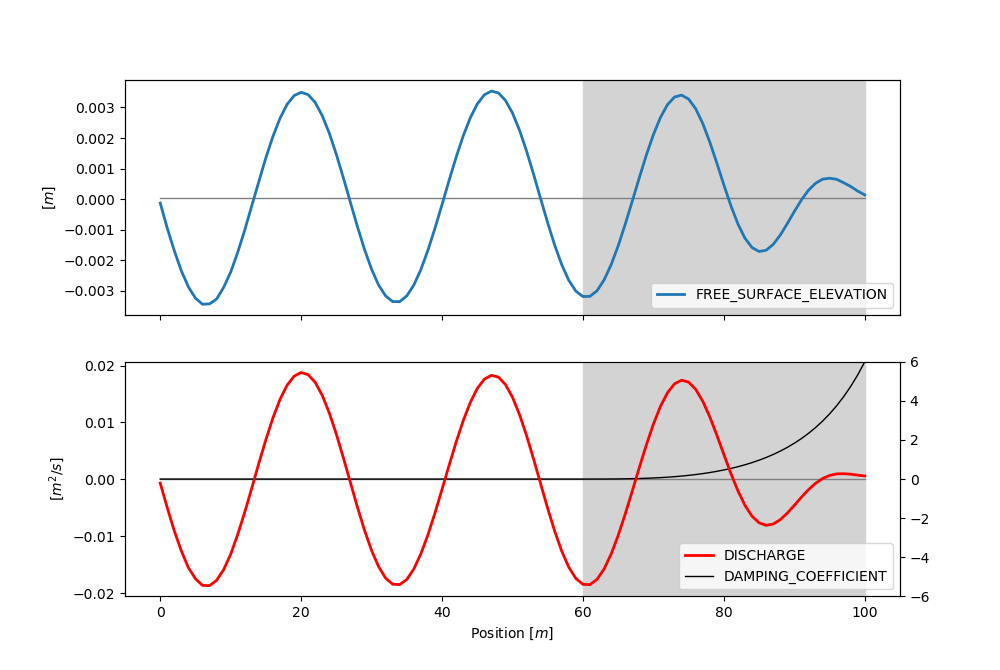
\includegraphics[width=.8\textwidth]{img/absorbing_boundary.png}
    \caption{Propagación y absorción de un tren de olas. La región sombreada de gris muestra el grosor de la capa esponja.}
    \label{absorbing_boundary}
\end{figure}


\subsection{Examples}



\section{Concluding remarks}


